\documentclass[a4paper, 11pt]{article}
\usepackage[UTF8]{ctex}
\usepackage[cpp]{mypackage}
\usepackage{float}
\usepackage{amsmath}
\usepackage{graphicx}
\usepackage{geometry}
\usepackage{listings}
\geometry{scale=0.8}
% \linespread{1.5}
\usepackage[colorlinks,linkcolor=red]{hyperref}

\title{	
\normalfont \normalsize
\textsc{School of Data and Computer Science, Sun Yat-sen University} \\ [25pt] %textsc small capital letters
\rule{\textwidth}{0.5pt} \\[0.4cm] % Thin top horizontal rule
\huge  T01 Search and Game Tree Search\\ % The assignment title
\rule{\textwidth}{2pt} \\[0.5cm] % Thick bottom horizontal rule
\author{17341015 陈鸿峥}
\date{\normalsize\today}
}

\begin{document}
\maketitle
\tableofcontents
\newpage

\section{Q1 - 环检测算法}
\begin{question}
使用\textbf{带环检测的一致代价搜索}寻找从Arad出发去Bucharest的路径,并作出搜索树。
% Consider travel in Romania from Arad to Bucharest. Trace the operation of uniform-cost search with cycle-checking: draw the search tree.
\end{question}
\begin{answer}
如下图所示,环检测部分已经用删除线标出。
注意每次添加进边界集的顺序以字母为序,但是扩展结点以路径代价为序。
\begin{figure}[H]
\centering
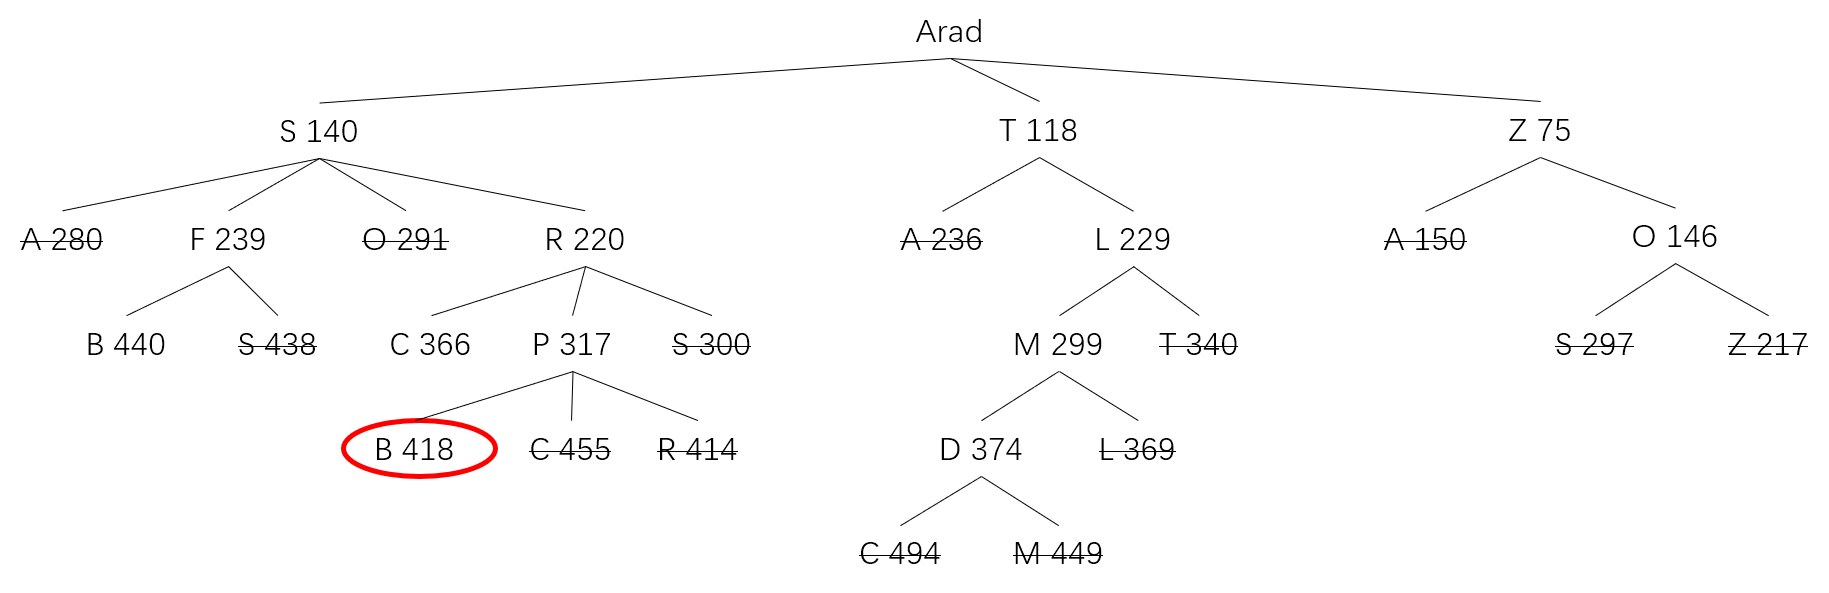
\includegraphics[width=\linewidth]{fig/A1.png}
\end{figure}
\end{answer}

\section{Q2 - $A^\star$算法}
\begin{question}[传教士与野人问题]
考虑$M=5$且$K=3$的情况,采用启发式函数$h(n)=M+C-2B$。
记录\textbf{带环检测的$A^\star$算法}的操作,作出搜索树;对于每一个结点,记录它的$g$和$h$值。
% The missionaries and cannibals problem (see the lecture notes): Consider the case of M = 5 and K = 3. Use the heuristic function h(n) = M + C − 2B. Trace the operation of $A^\star$ with cycle checking: Draw the search tree; for each node, mark its g and h values.
\end{question}
\begin{answer}
如下图所示,$g$值用铅笔写在右侧,$h$值写在每个元组的旁边。
\begin{figure}[H]
\centering
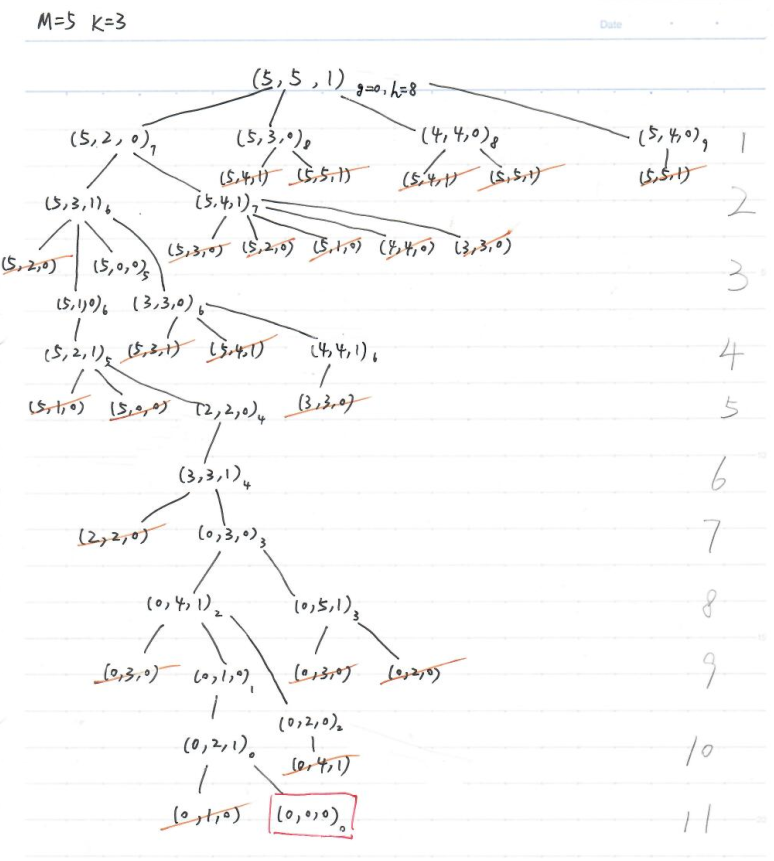
\includegraphics[width=\linewidth]{fig/A2-1.png}
\end{figure}
由于整个过程非常繁复,因此我也编程进行实现验证结果,如下图所示,其中括号内内容为当前启发式函数$f=g+h$的值,$d$则表示被环检测检测出来需要被剪枝的节点。
\begin{figure}[H]
\centering
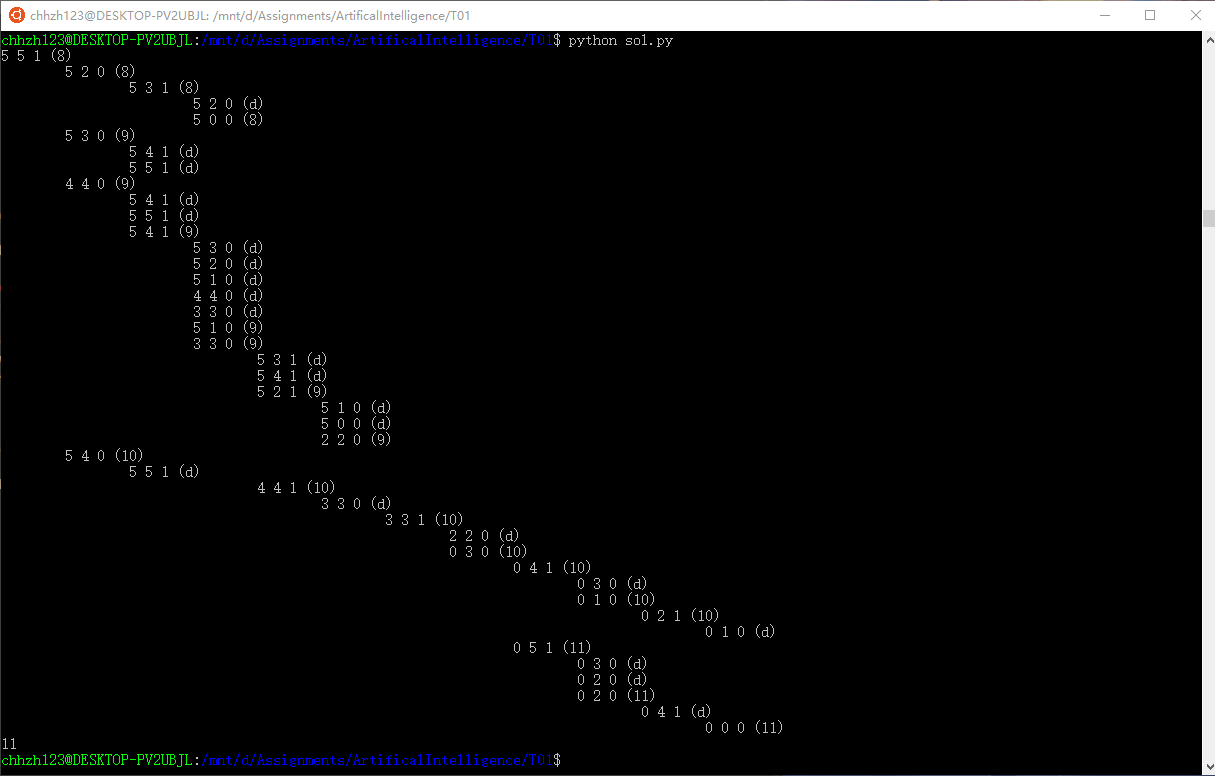
\includegraphics[width=\linewidth]{fig/program.png}
\end{figure}
可以看出结果确实正确,即使采用$A^\star$算法也需要经过11步才能找到最优解。
\end{answer}


\section{Q3 - $\alpha-\beta$剪枝}
\begin{question}
采用\textbf{$\alpha-\beta$剪枝}对下面的博弈树进行搜索,计算出根节点的效用。
% Perform alpha beta pruning on the following game tree and compute the utility value of the root.
\begin{figure}[H]
\centering
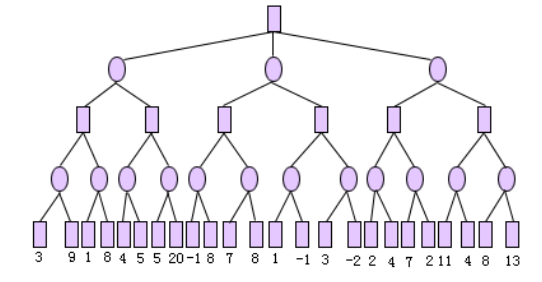
\includegraphics[width=\linewidth]{fig/Q3.png}
\end{figure}
\end{question}
\begin{answer}
如下图所示,剪枝部分已经用红色线标出。
\begin{figure}[H]
\centering
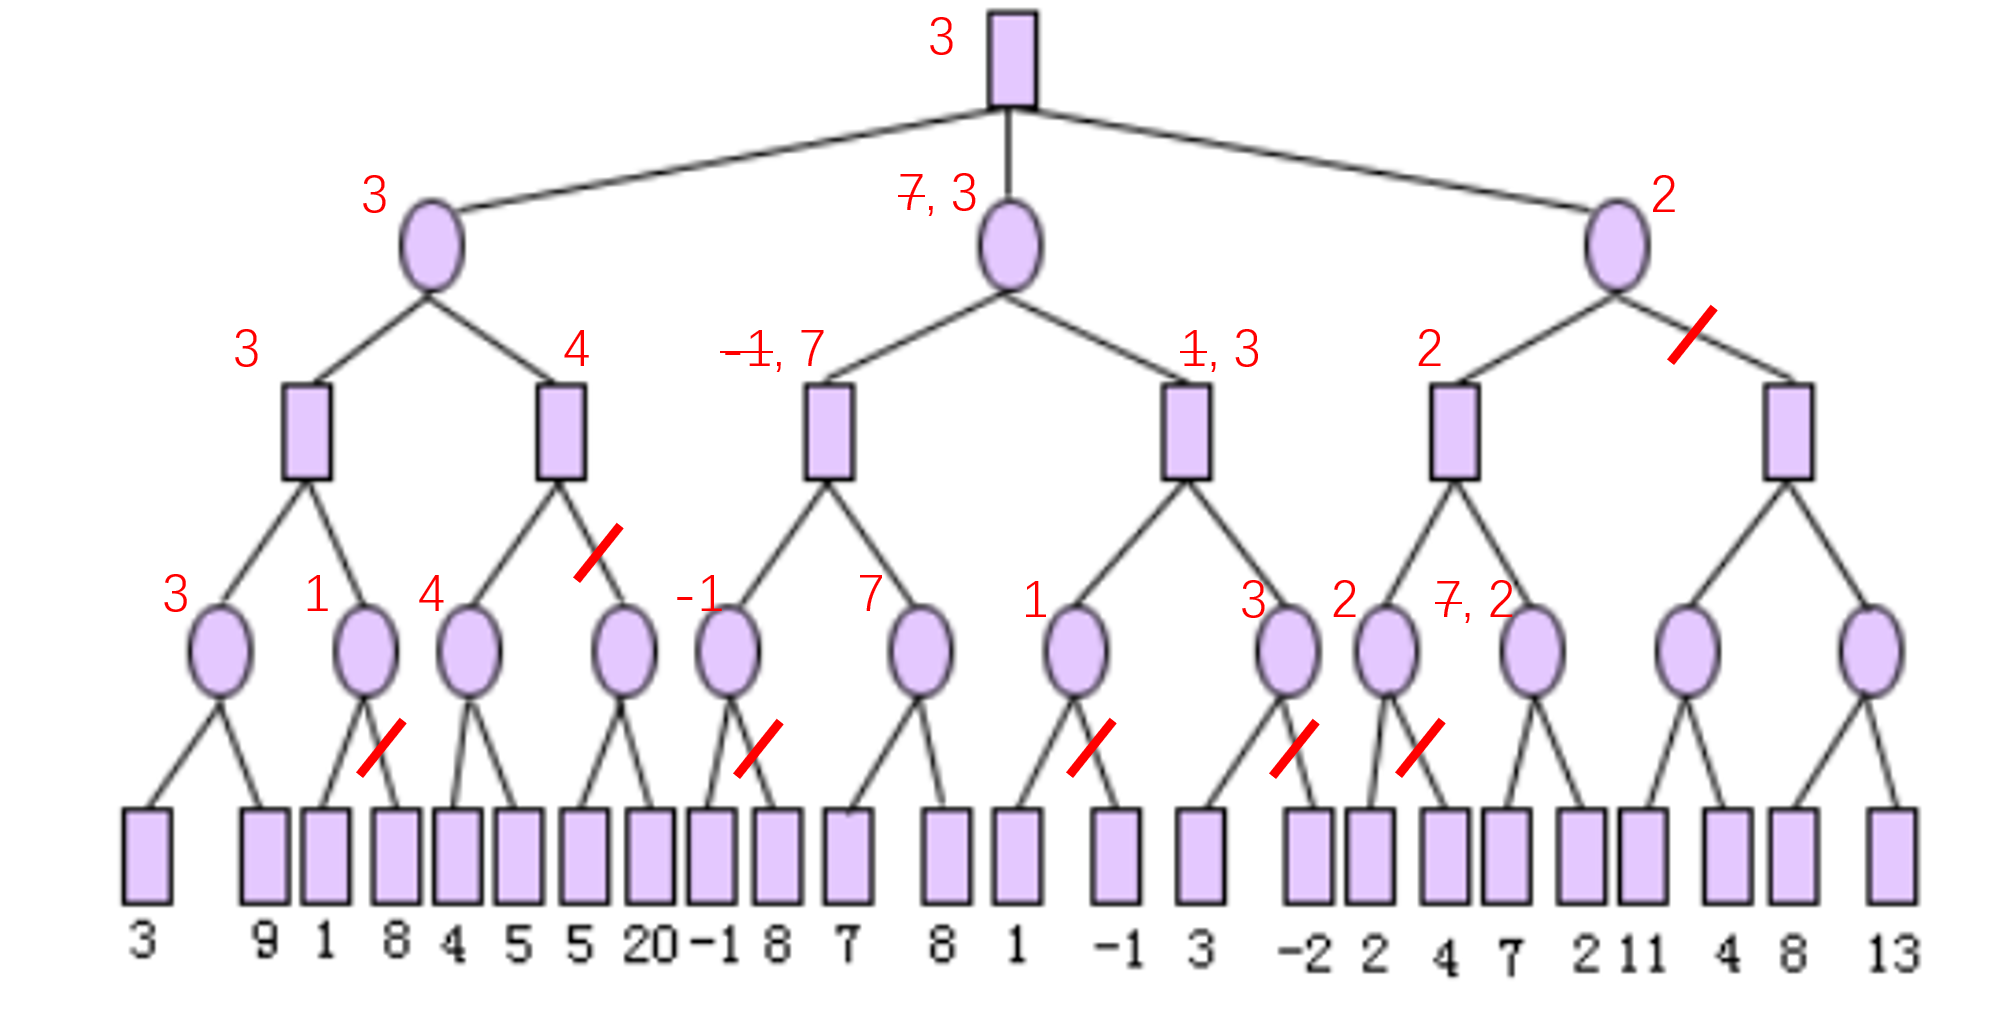
\includegraphics[width=\linewidth]{fig/A3.png}
\end{figure}
\end{answer}


\end{document}